\begin{apartats}

\begin{tria}{asimptotes-tasca}
\itemtria{original}{1}{1,25}
Troba totes les asímptotes de la funció
\[
f(x)=\frac{x^2+2}{x^2-x-2} .
\]

\begin{solucio}
\textbf{Verticals}: el denominador és $(x-2)(x+1)$, que s'anul·la en $x=2$ i en $x=-1$, i el numerador
no s'hi anul·la ($6$ i $3$). En $x=2$ els laterals valen $-\infty$ (per l'esquerra) i $+\infty$ (per
la dreta), i en $x=-1$, $+\infty$ i $-\infty$: asímptotes verticals $\boxed{x=2}$ i $\boxed{x=-1}$.\\
\textbf{Horitzontal}: numerador i denominador tenen el mateix grau, i
$\lim_{x\to\pm\infty}f(x)=\dfrac11=1$: asímptota horitzontal $\boxed{y=1}$. Per tant, no n'hi ha
cap d'obliqua.
\end{solucio}

\itemtria{talla-asimptota}{1}{1,25}
Troba les asímptotes de la funció
\[
f(x)=\frac{x^2+2x}{x^2+1} ,
\]
i estudia si la gràfica talla l'asímptota horitzontal. Una gràfica pot tallar una asímptota vertical?

\begin{solucio}
\textbf{Verticals}: cap, perquè el denominador, $x^2+1$, no s'anul·la mai.\\
\textbf{Horitzontal}: mateix grau, i $\lim_{x\to\pm\infty}f(x)=1$: $\boxed{y=1}$. Per tant, no n'hi ha
cap d'obliqua.\\
\textbf{Tall amb l'asímptota}: $f(x)=1$ si $x^2+2x=x^2+1$, és a dir si $x=\tfrac12$. La gràfica talla
l'asímptota horitzontal en $\left(\tfrac12,1\right)$: una asímptota horitzontal descriu el
comportament a l'infinit, i la gràfica la pot tallar en punts concrets.\\
Una asímptota vertical $x=a$ d'una funció racional, en canvi, no es pot tallar, perquè la funció no
està definida en $x=a$.
\end{solucio}
\end{tria}

\begin{nomesllarg}
\apartat{0,75}
Troba totes les asímptotes de la funció
\[
g(x)=\frac{2x^2-3x}{x+1} .
\]

\begin{solucio}
\textbf{Vertical}: $x=-1$, perquè el denominador s'hi anul·la i el numerador val $5\neq0$.\\
\textbf{Obliqua}: el grau del numerador supera en $1$ el del denominador. Dividint,
$\dfrac{2x^2-3x}{x+1}=2x-5+\dfrac{5}{x+1}$, i el terme que sobra tendeix a $0$: asímptota obliqua
$\boxed{y=2x-5}$. No hi ha asímptota horitzontal.
\end{solucio}
\end{nomesllarg}

\apartat[1,25]{0,75}
Dibuixa la gràfica d'una funció que tingui domini $\mathbb{R}\setminus\{0\}$, asímptota horitzontal
$y=1$ i asímptota vertical $x=0$, amb $\lim_{x\to0}f(x)=+\infty$ pels dos costats, i escriu-ne una
expressió.

\begin{solucio}
Per exemple, $f(x)=1+\dfrac{1}{x^2}$: el domini és $\mathbb{R}\setminus\{0\}$; com que $x^2>0$, els
dos laterals en $x=0$ valen $+\infty$ (l'asímptota vertical és l'eix $OY$); i
$\lim_{x\to\pm\infty}f(x)=1$.
\begin{center}
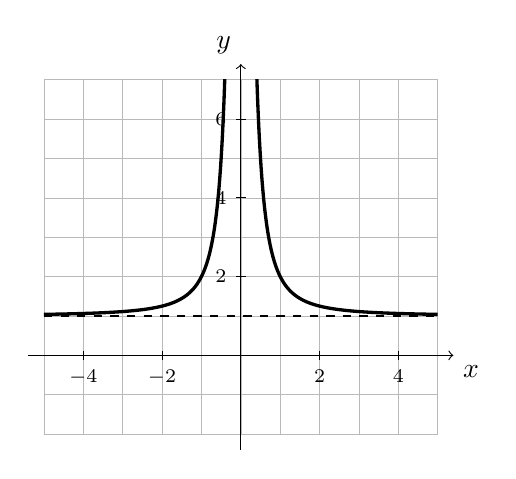
\begin{tikzpicture}[x=0.5cm,y=0.5cm]
  \draw[gray!55,very thin,step=1] (-5,-2) grid (5,7);
  \draw[->] (-5.4,0) -- (5.4,0) node[below right] {$x$};
  \draw[->] (0,-2.4) -- (0,7.4) node[above left] {$y$};
  \foreach \i in {-4,-2,2,4} \draw (\i,0.12) -- (\i,-0.12) node[below,font=\scriptsize] {$\i$};
  \foreach \j in {2,4,6} \draw (0.12,\j) -- (-0.12,\j) node[left,font=\scriptsize] {$\j$};
  \draw[dashed,thick] (-5,1) -- (5,1);
  \begin{scope}
    \clip (-5,-2) rectangle (5,7);
    \draw[\colorgrafica,very thick,domain=-5:-0.37,samples=100,smooth] plot (\x,{1+1/(\x*\x)});
    \draw[\colorgrafica,very thick,domain=0.37:5,samples=100,smooth] plot (\x,{1+1/(\x*\x)});
  \end{scope}
\end{tikzpicture}
\end{center}
Qualsevol altra funció amb aquestes propietats també val.
\end{solucio}

\end{apartats}
